\documentclass[14pt]{extarticle}
\usepackage{tikz}
\usepackage[top=0.25in, bottom=0.25in, left=0.25in, right=0.25in]{geometry}
\usepackage{xcolor}
\usetikzlibrary{arrows.meta}

\pagenumbering{gobble}

\newcommand{\blankbox}{\colorbox{pink}{\rule{22pt}{0pt}\rule{0pt}{22pt}}}

\title{Addition Exercises}
\author{}
\date{\Large\today}

\begin{document}

\maketitle

\noindent Name: \underline{\hspace{6cm}}
\vspace{1cm}

\begin{center}
\begin{tabular}{p{0.45\textwidth} p{0.45\textwidth}}

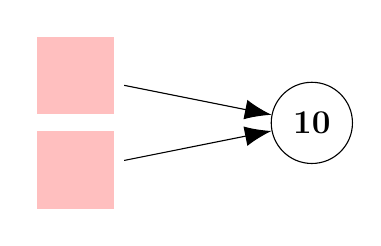
\begin{tikzpicture}[scale=3, every node/.style={font=\large\bfseries}]
% Problem 1
\node[circle,draw=black, fill=white, inner sep=5pt] (sum1) at (1, 0.7) {10};
\node (input11) at (0,0.9) {\blankbox};
\node (input12) at (0,0.5) {\blankbox};
\draw[-{Latex[scale=2.0]}] (input11) -- (sum1);
\draw[-{Latex[scale=2.0]}] (input12) -- (sum1);
\end{tikzpicture}
& 
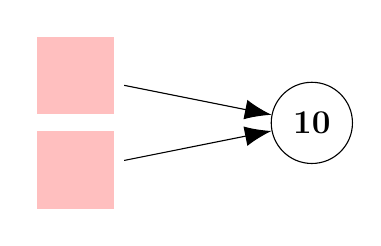
\begin{tikzpicture}[scale=3, every node/.style={font=\large\bfseries}]
% Problem 2
\node[circle,draw=black, fill=white, inner sep=5pt] (sum2) at (1, 0.7) {10};
\node (input21) at (0,0.9) {\blankbox};
\node (input22) at (0,0.5) {\blankbox};
\draw[-{Latex[scale=2.0]}] (input21) -- (sum2);
\draw[-{Latex[scale=2.0]}] (input22) -- (sum2);
\end{tikzpicture}

\\[0.5cm]

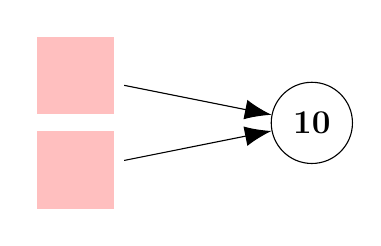
\begin{tikzpicture}[scale=3, every node/.style={font=\large\bfseries}]
% Problem 3
\node[circle,draw=black, fill=white, inner sep=5pt] (sum3) at (1, 0.7) {10};
\node (input31) at (0,0.9) {\blankbox};
\node (input32) at (0,0.5) {\blankbox};
\draw[-{Latex[scale=2.0]}] (input31) -- (sum3);
\draw[-{Latex[scale=2.0]}] (input32) -- (sum3);
\end{tikzpicture}
& 
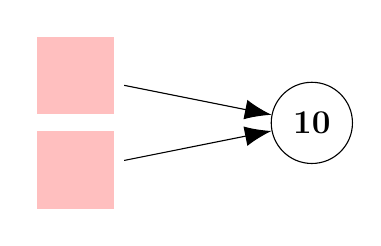
\begin{tikzpicture}[scale=3, every node/.style={font=\large\bfseries}]
% Problem 4
\node[circle,draw=black, fill=white, inner sep=5pt] (sum4) at (1, 0.7) {10};
\node (input41) at (0,0.9) {\blankbox};
\node (input42) at (0,0.5) {\blankbox};
\draw[-{Latex[scale=2.0]}] (input41) -- (sum4);
\draw[-{Latex[scale=2.0]}] (input42) -- (sum4);
\end{tikzpicture}

\\[0.5cm]

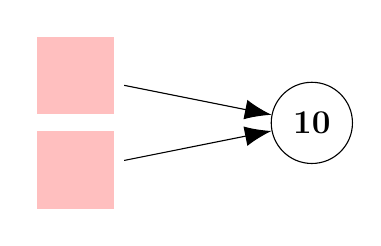
\begin{tikzpicture}[scale=3, every node/.style={font=\large\bfseries}]
% Problem 5
\node[circle,draw=black, fill=white, inner sep=5pt] (sum5) at (1, 0.7) {10};
\node (input51) at (0,0.9) {\blankbox};
\node (input52) at (0,0.5) {\blankbox};
\draw[-{Latex[scale=2.0]}] (input51) -- (sum5);
\draw[-{Latex[scale=2.0]}] (input52) -- (sum5);
\end{tikzpicture}
& 
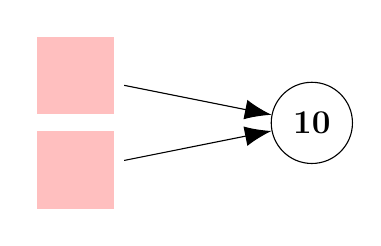
\begin{tikzpicture}[scale=3, every node/.style={font=\large\bfseries}]
% Problem 6
\node[circle,draw=black, fill=white, inner sep=5pt] (sum6) at (1, 0.7) {10};
\node (input61) at (0,0.9) {\blankbox};
\node (input62) at (0,0.5) {\blankbox};
\draw[-{Latex[scale=2.0]}] (input61) -- (sum6);
\draw[-{Latex[scale=2.0]}] (input62) -- (sum6);
\end{tikzpicture}

\\[0.5cm]

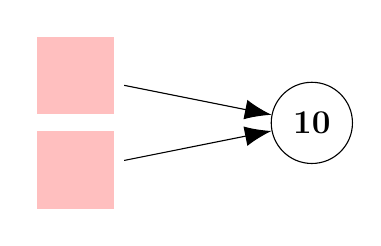
\begin{tikzpicture}[scale=3, every node/.style={font=\large\bfseries}]
% Problem 7
\node[circle,draw=black, fill=white, inner sep=5pt] (sum7) at (1, 0.7) {10};
\node (input71) at (0,0.9) {\blankbox};
\node (input72) at (0,0.5) {\blankbox};
\draw[-{Latex[scale=2.0]}] (input71) -- (sum7);
\draw[-{Latex[scale=2.0]}] (input72) -- (sum7);
\end{tikzpicture}
& 
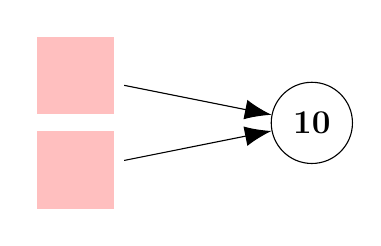
\begin{tikzpicture}[scale=3, every node/.style={font=\large\bfseries}]
% Problem 8
\node[circle,draw=black, fill=white, inner sep=5pt] (sum8) at (1, 0.7) {10};
\node (input81) at (0,0.9) {\blankbox};
\node (input82) at (0,0.5) {\blankbox};
\draw[-{Latex[scale=2.0]}] (input81) -- (sum8);
\draw[-{Latex[scale=2.0]}] (input82) -- (sum8);
\end{tikzpicture}

\\[0.5cm]

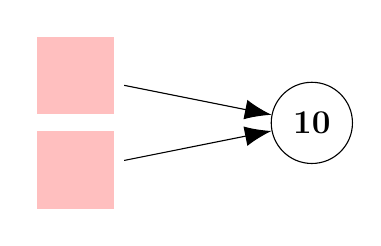
\begin{tikzpicture}[scale=3, every node/.style={font=\large\bfseries}]
% Problem 9
\node[circle,draw=black, fill=white, inner sep=5pt] (sum9) at (1, 0.7) {10};
\node (input91) at (0,0.9) {\blankbox};
\node (input92) at (0,0.5) {\blankbox};
\draw[-{Latex[scale=2.0]}] (input91) -- (sum9);
\draw[-{Latex[scale=2.0]}] (input92) -- (sum9);
\end{tikzpicture}
& 
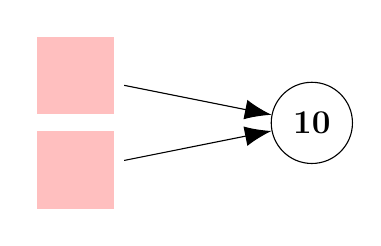
\begin{tikzpicture}[scale=3, every node/.style={font=\large\bfseries}]
% Problem 10
\node[circle,draw=black, fill=white, inner sep=5pt] (sum10) at (1, 0.7) {10};
\node (input101) at (0,0.9) {\blankbox};
\node (input102) at (0,0.5) {\blankbox};
\draw[-{Latex[scale=2.0]}] (input101) -- (sum10);
\draw[-{Latex[scale=2.0]}] (input102) -- (sum10);
\end{tikzpicture}

\end{tabular}
\end{center}

\end{document}
